\section{Problem 5}
\label{sec:problem5}

The longitudes of the ascending node are not given, so both orbits can be assumed to have $\Omega_1=\Omega_2=0$. The LEO radius can be found with the altitude:
\begin{equation*}
r_1 = R_E + 350~\text{km} = 6728~\text{km}, \qquad r_2 = 26558~\text{km}, \qquad \Omega_1 = \Omega_2 = 0
\end{equation*}

\subsection*{(a) and (b) Line of intersection and impulse positions}
The angular momentum directions, the line of intersection, and the impulse positions can be found in the course notes:
\begin{equation*}
\hat{\vect{h}}_k = \sin i_k\sin\Omega_k\,\vect{I}_x - \sin i_k\cos\Omega_k\,\vect{I}_y + \cos i_k\,\vect{I}_z
\end{equation*}
\begin{equation*}
\vect{\ell} = \frac{\ivect{h}_1\times\ivect{h}_2}{\|\ivect{h}_1\times\ivect{h}_2\|}
\end{equation*}
\begin{equation*}
\vect{r}_1 = r_1\vect{\ell}, \qquad \vect{r}_2 = -r_2\vect{\ell}
\end{equation*}

\subsection*{(c) Total $\Delta V$}
We can find $\Delta V$ using the transfer orbit semi-major axis and the first and second impulses:
\begin{equation*}
a = \frac{r_1+r_2}{2}
\end{equation*}
\begin{equation*}
\Delta v_1 = \sqrt{\frac{2\mu}{r_1}-\frac{\mu}{a}} - \sqrt{\frac{\mu}{r_1}}
\end{equation*}
\begin{equation*}
\Delta v_2 = \sqrt{(v_2^-)^2 + (v_2^+)^2 - 2v_2^-v_2^+\cos\theta}, \qquad
v_2^- = \sqrt{\frac{2\mu}{r_2}-\frac{\mu}{a}}, \qquad v_2^+ = \sqrt{\frac{\mu}{r_2}}
\end{equation*}
The rotation angle $\theta$ follows from
\begin{equation*}
\cos\theta = \hat{\vect{h}}_1\cdot\hat{\vect{h}}_2
= \sin i_1\sin i_2\left(\sin\Omega_1\sin\Omega_2 + \cos\Omega_1\cos\Omega_2\right) + \cos i_1\cos i_2
\end{equation*}
This reduces to $i_2-i_1$ because $\Omega_1=\Omega_2$:
\begin{align*}
\cos\theta &= \sin i_1\sin i_2\left(\sin^2\Omega_1 + \cos^2\Omega_1\right) + \cos i_1\cos i_2 \\
&= \cos i_1\cos i_2 + \sin i_1\sin i_2 = \cos(i_2-i_1)
\;\Rightarrow\; \theta = i_2 - i_1
\end{align*}
And thus:
\begin{equation*}
\boxed{\Delta V = \Delta v_1 + \Delta v_2
= \sqrt{\frac{2\mu}{r_1}-\frac{\mu}{a}} - \sqrt{\frac{\mu}{r_1}}
+ \sqrt{(v_2^-)^2 + (v_2^+)^2 - 2v_2^-v_2^+\cos(i_2-i_1)}}
\end{equation*}

\subsection*{(d), (e), and (f) Time of flight, eccentricity, and plane rotation angle}
The time of flight is half the transfer orbit's period, eccentricity can be found with the initial and terminal radii, and the rotation angle is $\theta$, given above:
\begin{equation*}
t_f = \pi\sqrt{\frac{a^3}{\mu}}, \qquad
e = \frac{r_2-r_1}{r_2+r_1}
\end{equation*}

\medskip
\noindent The expressions in parts (a) through (f) are evaluated in \texttt{problem5.py} with $\mu = 398600~\text{km}^3/\text{s}^2$ and $R_E = 6378$~km, giving:

\medskip
\programoutput{outputs/problem5.txt}

\subsection*{(g) Transfer plot}

\begin{figure}[H]
\centering
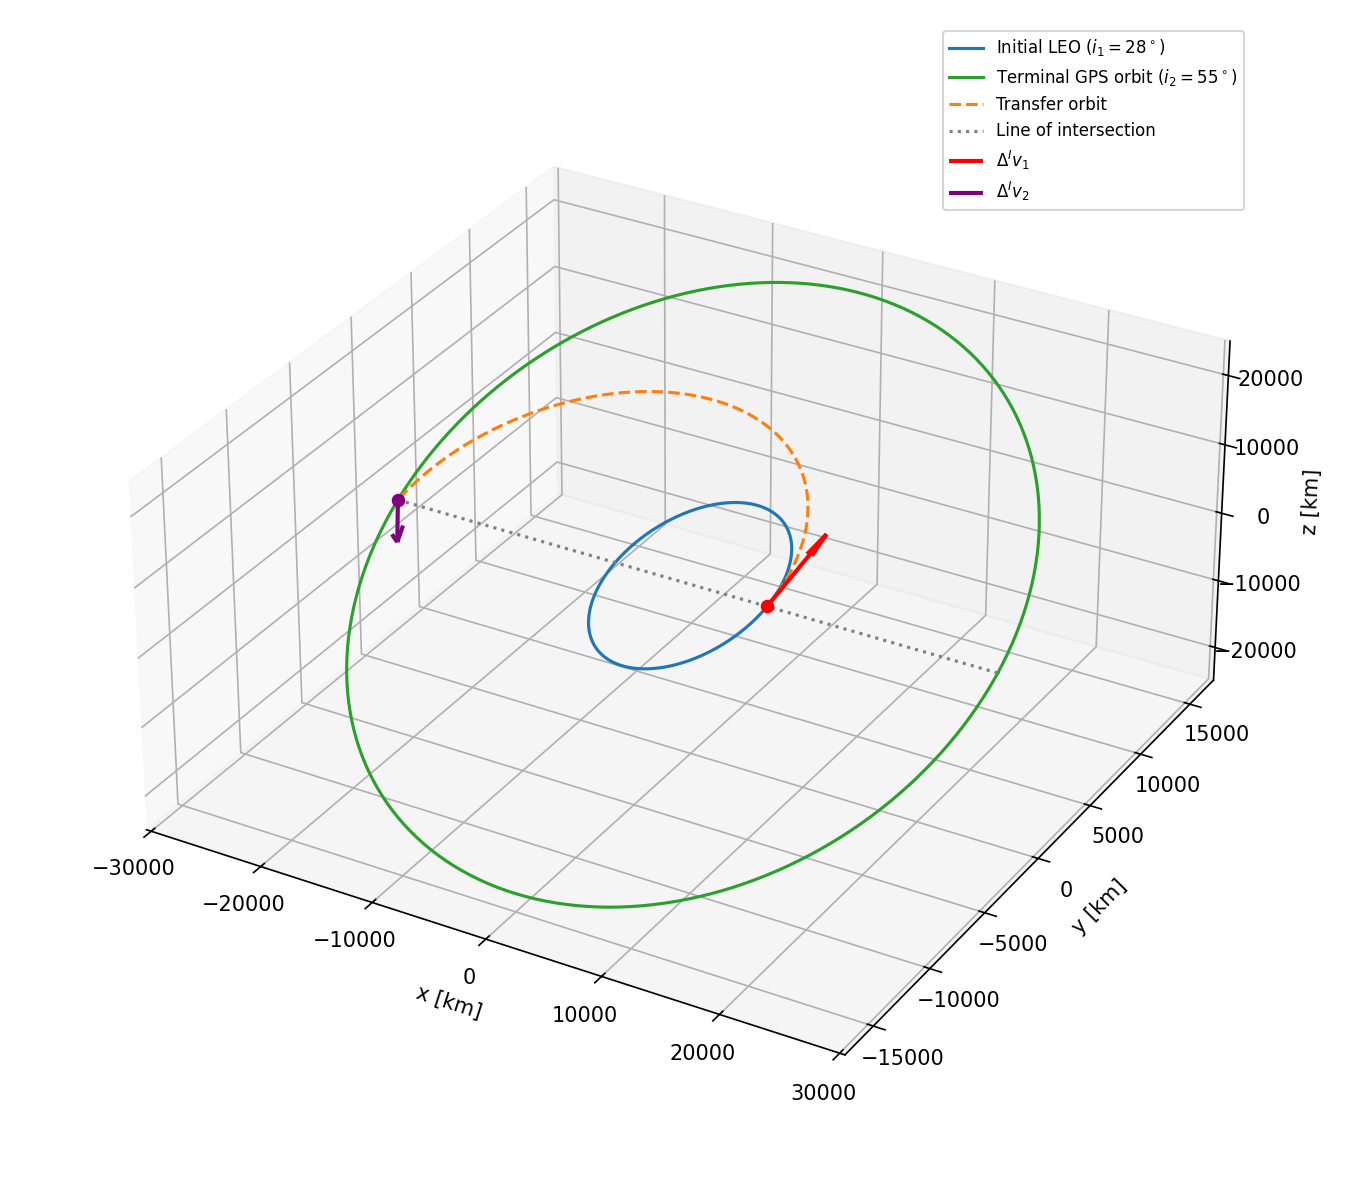
\includegraphics[width=0.8\textwidth]{problem5_transfer.png}
\caption{Two-impulse LEO-to-GPS transfer with both impulses on the line of intersection.}
\label{fig:p5-transfer}
\end{figure}

\FloatBarrier
